\documentclass[a4paper,10pt, oneside, titlepage]{article}

\usepackage[spanish,es-tabla]{babel}
\usepackage[hidelinks]{hyperref}
\usepackage[utf8]{inputenc}
\usepackage[T1]{fontenc}
\usepackage{subcaption}
\usepackage{graphicx}
\usepackage{listings}
\usepackage{sectsty}
\usepackage{xcolor}

\title{Manual de Usuario Aplicación Android del Agente de Respuesta SIGOAVE}
\author{Arroyo Auz Christian Xavier}

\begin{document}
	\maketitle
	\section{Introducción}
	El agente de respuesta forma parte de un conjunto de sistemas autónomos para la gestión de accidentabilidad vehicular.\\\\
	El agente de respuesta se encarga de solicitar información procesada al servicio de siniestrabilidad vehicular (SIGOAVE).\\\\
	El agente de respuesta es una aplicación móvil que presenta el índice de accidentabilidad del vehículo y ciertos parámetros claves del conductor, vehículo, condiciones climatológicas y del flujo de tráfico que sustentan ese índice.\\\\
	Además, la aplicación genera notificaciones y alertas en base a la información provista por SIGOAVE.\\\\
	Una de las principales características de esta aplicación móvil es que funcione de manera autónoma, pero pueda trabajar en sinergia con la aplicación móvil del agente de adquisición.\\\\
	La Figura 1 presenta el esquema de este conjunto de sistemas autónomos.
	\begin{figure}[!h]
		\centering
		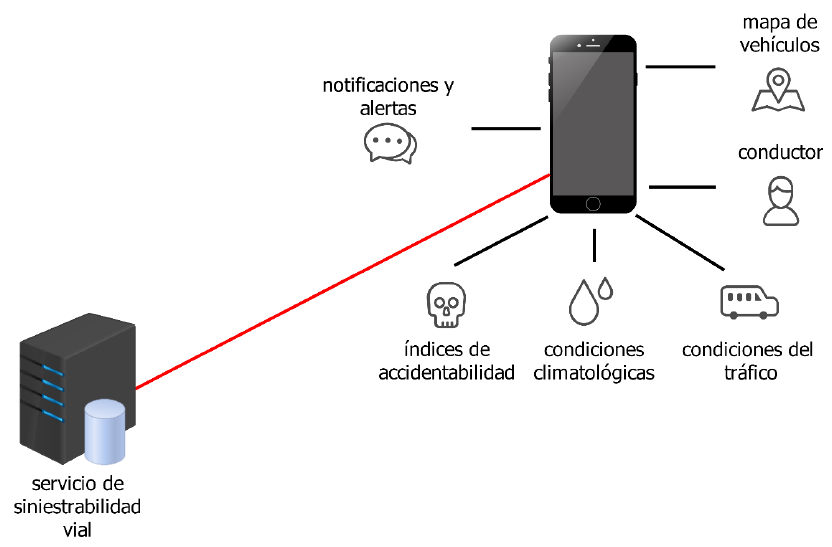
\includegraphics[width = 1\linewidth, height = 11.4cm]{1.png}
		\caption{Funcionalidades del Agente de Respuesta.}
	\end{figure}
	
	\section{Objetivos}
	\begin{itemize}
		\item Presentar la interfaz gráfica de usuario (GUI) de la aplicación móvil que conforma el agente de respuesta.
		\item Determinar mejoras a funcionalidades existentes y establecer funcionalidades nuevas que podrán ser incluidas en la aplicación.
		\item Desarrollar e implementar la aplicación móvil considerando los riesgos de seguridad definidos en la fase de diseño.
		\item Establecer los parámetros claves de cada una de las fuentes de datos (conductor, vehículo, condiciones meteorológicas y flujo de tráfico).
	\end{itemize}
	
	\section{Alcance}
	\begin{itemize}
		\item La aplicación móvil del agente de respuesta incluye lo siguiente:
		\item Una pantalla o “activity” para gestionar el inicio de sesión por medio de credenciales (nombre de usuario y contraseña).
		\item Pantallas para presentar los siguientes parámetros claves:
		\begin{itemize}
			\item Vehículo: velocidad, revoluciones por minuto, nivel de gasolina, temperatura del motor y ángulo de inclinación del volante.
			\item Condiciones meteorológicas: lugar o zona, temperatura, precipitación, humedad, y velocidad del viento.
			\item Flujo de tráfico: ubicación, velocidad promedio, número de vehículos, ocupación promedio y dirección del flujo.
			\item Conductor: edad, genero, uso de lentes, estado de licencia y puntos disponibles, y condiciones médicas.
		\end{itemize}
		\item Una pantalla que incluye un mapa para ubicar los vehículos que se encuentran en la zona.
		\item Cada una de las pantallas presenta como encabezado información relacionada al índice de accidentabilidad.
	\end{itemize}

	\section{Requerimientos de la APP}
	\subsection{Requerimientos Funcionales}
	\begin{itemize}
		\item Proveer un mecanismo para iniciar sesión en el servicio de siniestrabilidad vial.
		\item Consultar periódicamente información al servicio.
		\item Mostrar información del conductor, índices de accidentabilidad y otros parámetros del vehículo (velocidad, rpm, etc.).
		\item Presentar alertas de los índices de siniestrabilidad.
		\item Presentar notificaciones de las condiciones meteorológicas y condiciones del tráfico.
		\item Mostrar estadísticas de varios parámetros.
		\item Compartir información como índices de accidentabilidad con vehículos registrados en el servicio.
		\item Implementar una función de actualización automática para información relacionada a índices de accidentabilidad, condiciones meteorológicas y condiciones de tráfico.
		\item Presentar un mapa de ubicación de vehículos en función de la cercanía.
		\item Funcionar en forma independiente al funcionamiento de la aplicación móvil (agente de adquisición).
		\item Ser implementado considerando los siguientes riesgos de seguridad: uso inadecuado de la plataforma, comunicación insegura, autenticación insegura y criptografía insuficiente.
	\end{itemize}
	\subsection{Requerimientos No Funcionales}
	\begin{itemize}
		\item Iniciar sesión en el servicio de siniestrabilidad por medio de credenciales o a través del lector de huellas dactilares.
		\item Consultar resultados una vez que estén disponibles en el servicio de accidentabilidad.
		\item Presentar alertas visuales y auditivas cuando el índice de siniestrabilidad supere un valor umbral.
		\item Presentar notificaciones de condiciones climatológicas y de tráfico en la medida que estos cambien repentinamente su valor.
	\end{itemize}
	
	\section{Instalación de la aplicación}
	Dado que la aplicación aún no se encuentra establecida en la Play Store, esta se debe obtener de forma manual desde el repositorio del creador.\\\\
	Página de Descarga: \textcolor{blue}{\url{https://www.epn.edu.ec/app/sigoave}}
	\subsection{Instalación de la aplicación desde PC}
	Una vez descargada la APP desde la página web del creador, se debe proceder a descargar e instalar un software que permita la instalación de archivos APK desde el computador. Se recomienda usar ``Pure APK Install''.\\\\
	Página de Descarga: \textcolor{blue}{\url{https://apkpure.com/es/apk-install.html}}\\\\
	Pure APK Install es un software de instalación de APK para Android, desarrollado por el equipo de APK Pure. Con esta herramienta de instalación de APK, puede instalar fácilmente juegos y aplicaciones APK desde la PC al teléfono o tableta Android.\\\\
	Instalado el software, se procede a habilitar las opciones de desarrollador en el dispositivo celular el cual se desea instalar la aplicación, como se muestra en la Figura 2.
	\begin{figure}[!h]
		\centering
		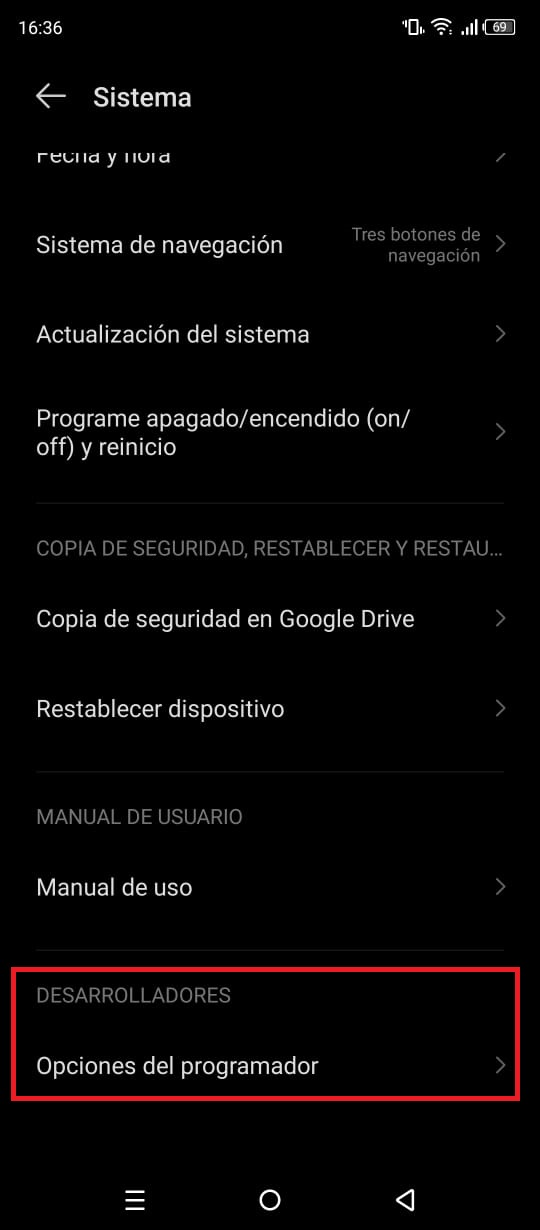
\includegraphics[width = 0.45\linewidth, height = 9cm]{2.jpeg}
		\caption{Activación del Modo Desarrollador.}
	\end{figure}\\
	En Android 4.1 y versiones anteriores, la pantalla Opciones para desarrolladores está disponible de forma predeterminada. En Android 4.2 y versiones posteriores, debes habilitarla. Esto puede variar según el dispositivo pero normalmente se realiza los siguientes paso:
	\begin{itemize}
		\item En tu dispositivo, busca la opción Número de compilación:
		\begin{itemize}
			\item Opción 1: Configuración $\rightarrow$ Acerca del teléfono $\rightarrow$ Número de compilación.
			\item Opción 2: Configuración $\rightarrow$ Acerca del teléfono $\rightarrow$ Información de software $\rightarrow$ Número de compilación.
			\item Opción 3: Configuración $\rightarrow$ Acerca del teléfono $\rightarrow$ Información de software $\rightarrow$ Número de compilación.
			\item Opción 4: Configuración $\rightarrow$ Acerca de $\rightarrow$ Información de software $\rightarrow$ Más $\rightarrow$ Número de compilación o Configuración $\rightarrow$ Sistema $\rightarrow$ Acerca del teléfono $\rightarrow$ Información de software $\rightarrow$ Más $\rightarrow$ Número de compilación.
			\item Opción 5: Configuración $\rightarrow$ Acerca del teléfono $\rightarrow$ Número de compilación.
		\end{itemize}
		\item Presiona la opción Número de compilación siete veces hasta que veas el mensaje ``Ahora eres desarrollador!''. Esto habilita las opciones para desarrolladores en tu dispositivo.
		\item Cuando regreses a la pantalla anterior, verás las Opciones para desarrolladores en la parte inferior.
	\end{itemize}
	Para poder usar el depurador y otras herramientas, debes habilitar la depuración por USB, que permite que Android y otras herramientas del SDK reconozcan tu dispositivo cuando se conecta mediante USB.\\\\
	Habilita la opción Depuración por USB en la configuración del sistema del dispositivo que se encuentra en Opciones para desarrolladores, como se muestra en la Figura 3.
	\begin{figure}[!h]
		\centering
		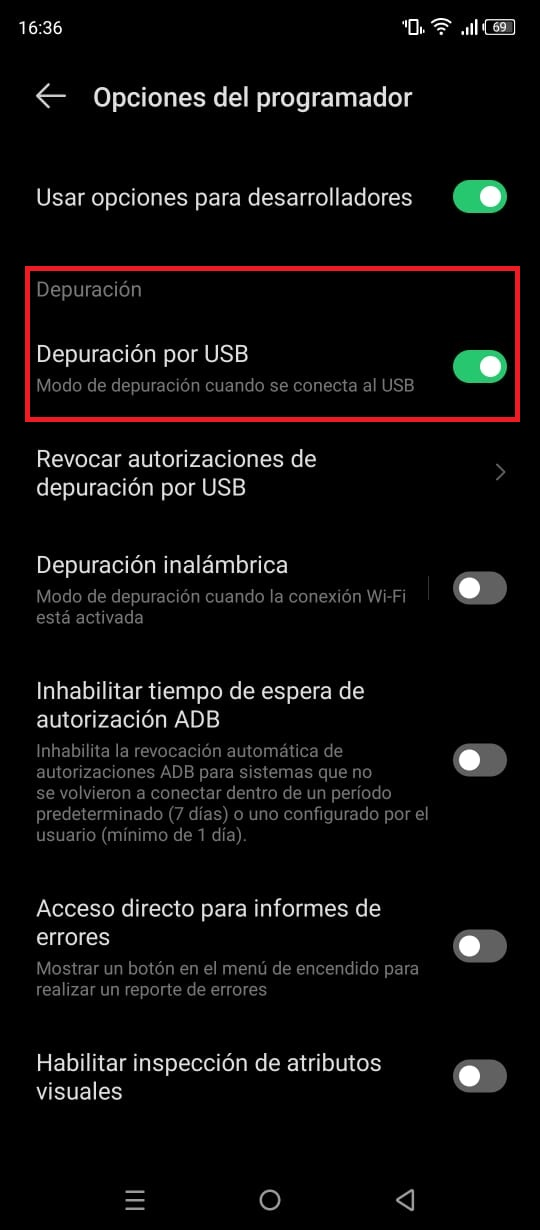
\includegraphics[width = 0.45\linewidth, height = 9cm]{3.jpeg}
		\caption{Activación de la Depuración por USB.}
	\end{figure}\\
	Puedes encontrar esta opción en una de las siguientes ubicaciones, según tu versión de Android:
	\begin{itemize}
		\item Android 9 (nivel de API 28) y versiones posteriores: Configuración $\rightarrow$ Sistema $\rightarrow$ Avanzado $\rightarrow$ Opciones para desarrolladores $\rightarrow$ Depuración por USB.
		\item Android 8.0.0 (nivel de API 26) y Android 8.1.0 (nivel de API 27): Configuración $\rightarrow$ Sistema $\rightarrow$ Opciones para desarrolladores $\rightarrow$ Depuración por USB.
		\item Android 7.1 (nivel de API 25) y versiones anteriores: Configuración $\rightarrow$ Opciones para desarrolladores $\rightarrow$ Depuración por USB.
	\end{itemize}
	Habilitada la Depuración por USB, se procede a iniciar el software de instalación, como se muestra en la Figura 4 y se procede a conectar el dispositivo celular al PC. Si el dispositivo celular muestra un mensaje de alerta como aprecia en la Figura 5, se debe conceder los permisos que este solicita.
	\begin{figure}[!h]
		\centering
		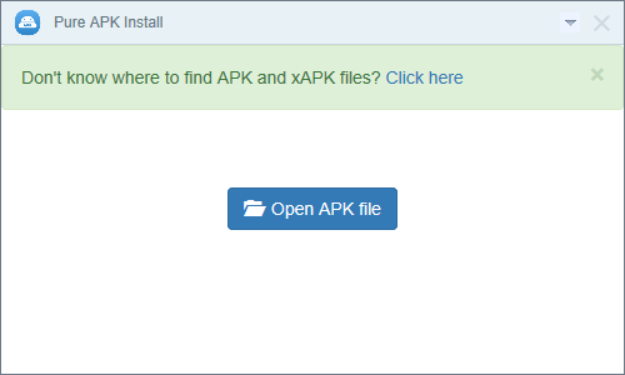
\includegraphics[width = 0.7\linewidth, height = 4.5cm]{4.png}
		\caption{Software de instalación iniciado.}
	\end{figure}
	\begin{figure}[!h]
		\centering
		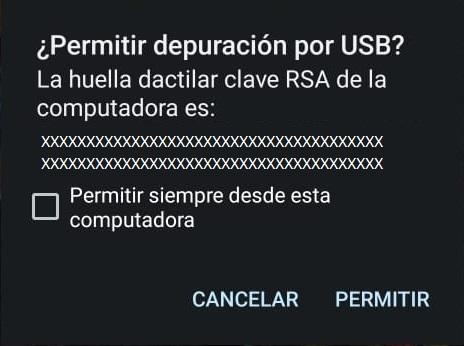
\includegraphics[width = 0.7\linewidth, height = 4.5cm]{5.jpeg}
		\caption{Solicitud de Depuración por USB.}
	\end{figure}\\
	Dentro del software de instalación se procede a cargar el APK desde su ubicación presionando el botón ``Open APK file'' y posteriormente buscándolo en su ubicación, como se observa en la Figura 6.
	\begin{figure}[!h]
		\centering
		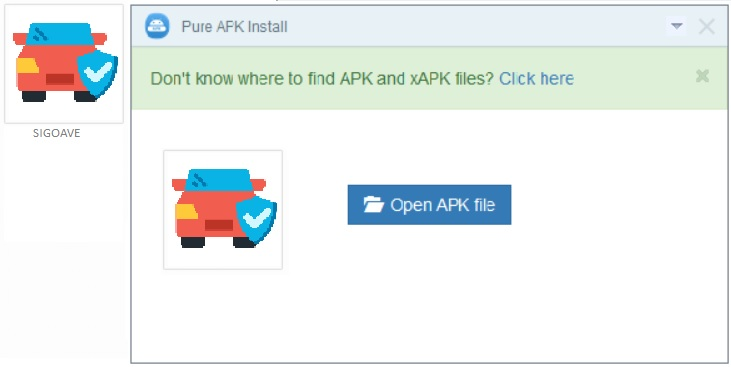
\includegraphics[width = 0.7\linewidth, height = 4.5cm]{6.jpg}
		\caption{Carga del APK.}
	\end{figure}\\
	Posteriormente, se procede a elegir el lugar de instalación de la APP. Se puede elegir entre el almacenamiento externo, almacenamiento interno o permitir que el software elija donde instalar la APP. Ver Figura 7.
	\begin{figure}[h]
		\centering
		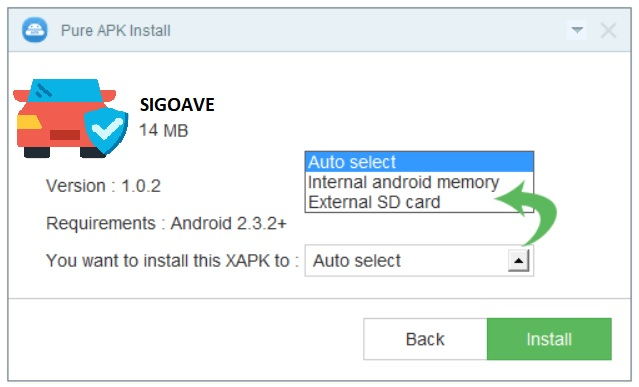
\includegraphics[width = 0.7\linewidth, height = 4.5cm]{7.jpg}
		\caption{Escogiendo el lugar de instalación.}
	\end{figure}\\
	Finalmente, se presiona en ``Instalar'' y se verifica que se la APP este instalada en el dispositivo celular. Ver Figura 8.
	\begin{figure}[h]
		\centering
		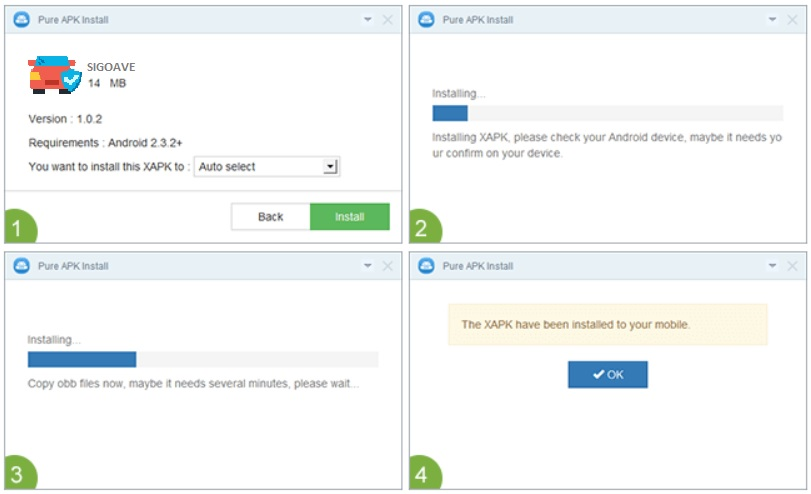
\includegraphics[width = 0.7\linewidth, height = 4.5cm]{8.jpg}
		\caption{Proceso de instalación.}
	\end{figure}
	
	\subsection{Instalación de la aplicación desde el celular}
	Este es el procedimiento más recomendado para realizar la instalación de la APP, ya que el proceso antes mencionado, ``Instalación de la aplicación desde PC'', puede provocar una serie de errores y conflictos difíciles de corregir sin experiencia en el manejo de software.\\\\
	Dado que la aplicación aún no se encuentra establecida en la Play Store, esta se debe obtener de forma manual desde el repositorio del creador.\\\\
	Página de Descarga: \textcolor{blue}{\url{https://www.epn.edu.ec/app/sigoave}}\\\\
	Descargada la APP desde el repositorio del creador, se debe abrir la carpeta donde se descargo la APP, normalmente de encuentra en la carpeta de ``Descargas''. Ver Figura 9.
	\begin{figure}[!h]
		\centering
		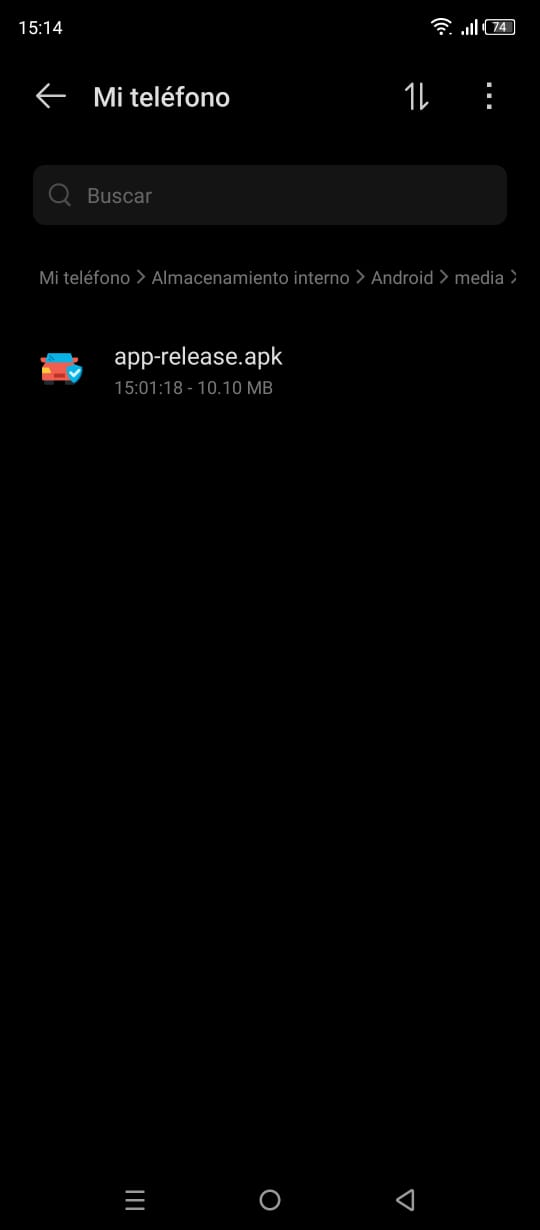
\includegraphics[width = 0.45\linewidth, height = 8.5cm]{9.jpeg}
		\caption{Ubicación del APK de instalación.}
	\end{figure}\\
	Ya en la ubicación del archivo se presiona sobre el icono del APK para proceder con la instalación. Si el celular solicita permisos, estos deben ser concedidos como se muestra en la Figura 10 y Figura 11.
	\begin{figure}[!h]
		\centering
		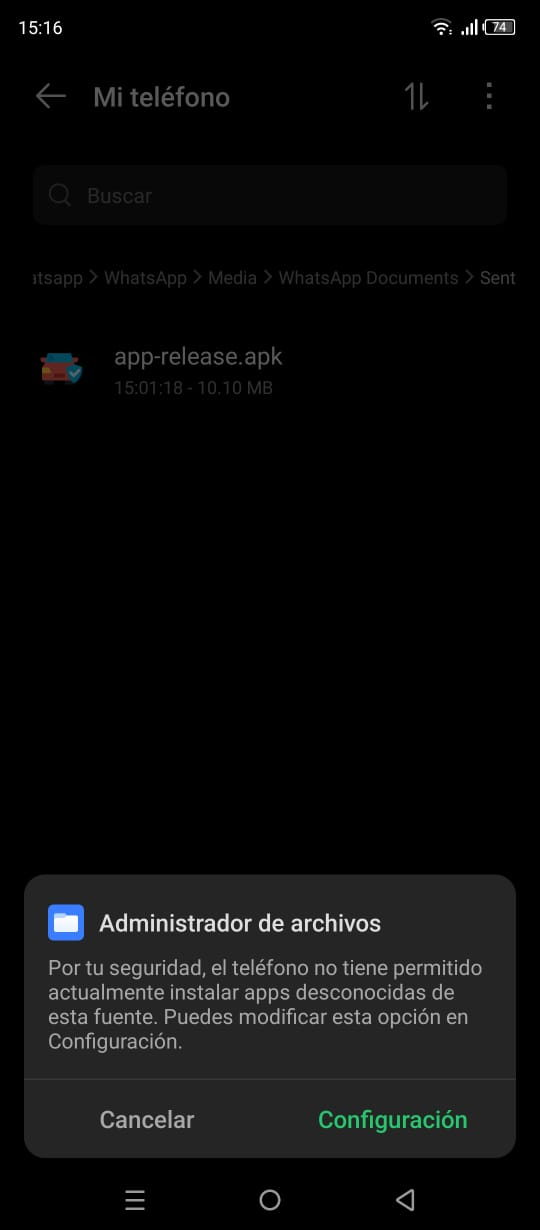
\includegraphics[width = 0.45\linewidth, height = 8.5cm]{10.jpeg}
		\caption{Configuración para instalación.}
	\end{figure}
	\begin{figure}[!h]
		\centering
		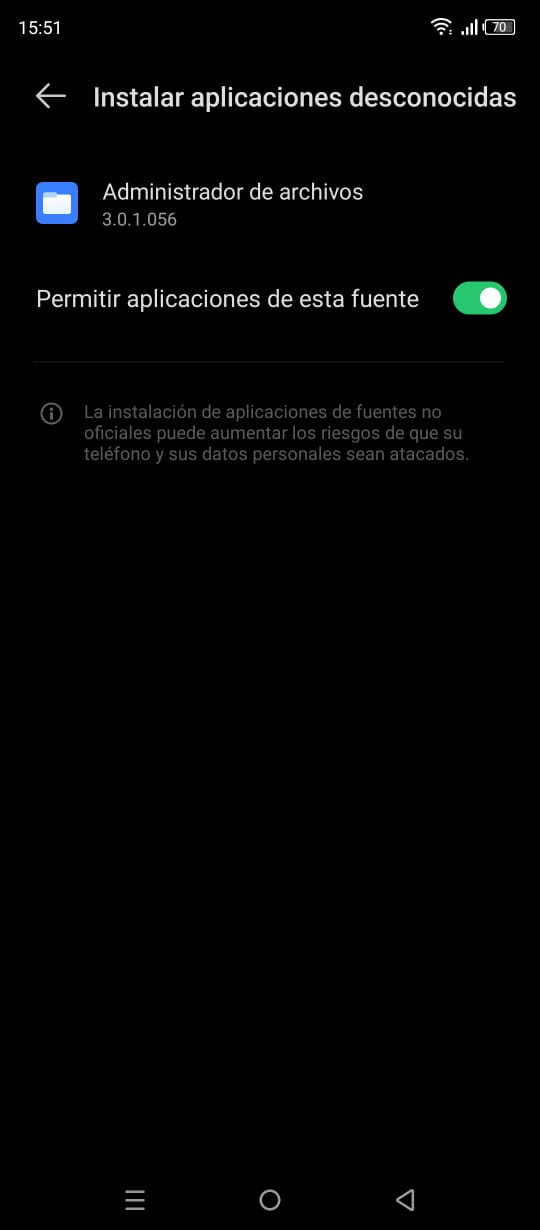
\includegraphics[width = 0.45\linewidth, height = 8.3cm]{11.jpeg}
		\caption{Concesión de permisos.}
	\end{figure}\\
	Posteriormente, se debe presionar en ``Instalar'', ver Figura 12.
	\begin{figure}[!h]
		\centering
		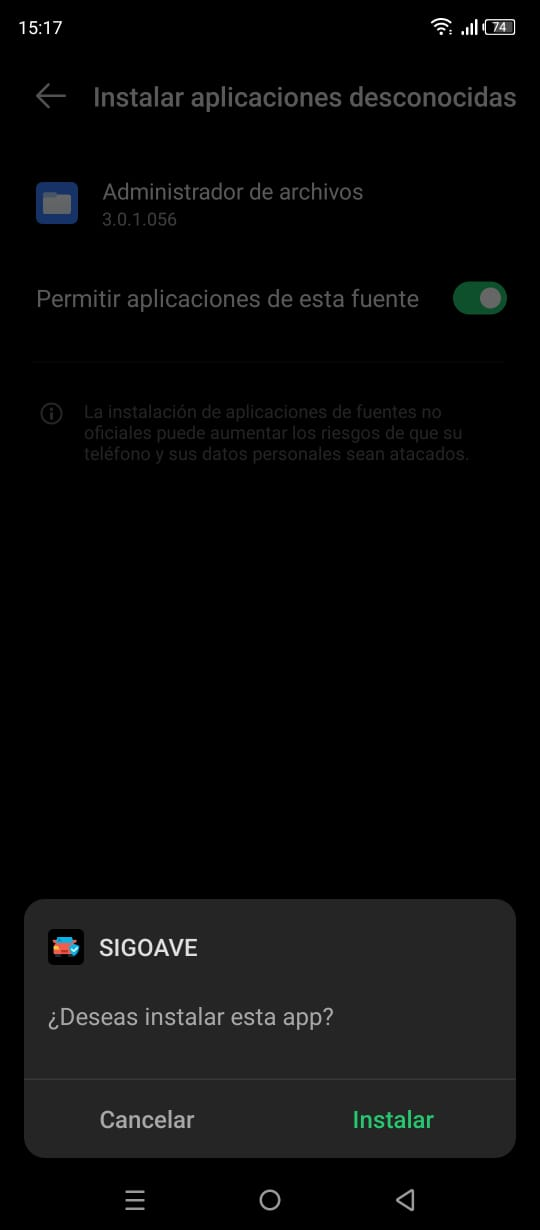
\includegraphics[width = 0.45\linewidth, height = 8.3cm]{12.jpeg}
		\caption{Inicio de proceso de instalación.}
	\end{figure}\\
	Es posible que la APP sea bloqueada por los servicios de Google, como muestra la Figura 13. En este caso se debe presionar en la opción de ``Instalar de todas formas''.
	\begin{figure}[!h]
		\centering
		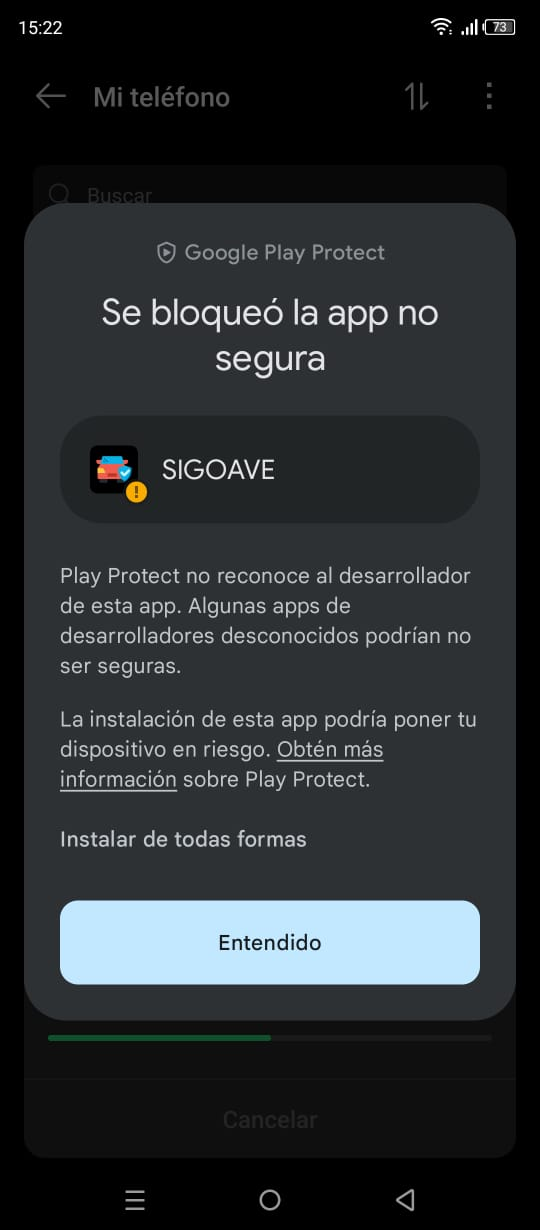
\includegraphics[width = 0.45\linewidth, height = 8.5cm]{13.jpeg}
		\caption{Forzar la instalación de la APP.}
	\end{figure}\\
	Finalmente, se puede observar un mensaje en el cual se informa que la APP fue instalada en el dispositivo. Ver Figura 14. En este punto se debe presionar en la opción ``Listo''.
	\begin{figure}[!h]
		\centering
		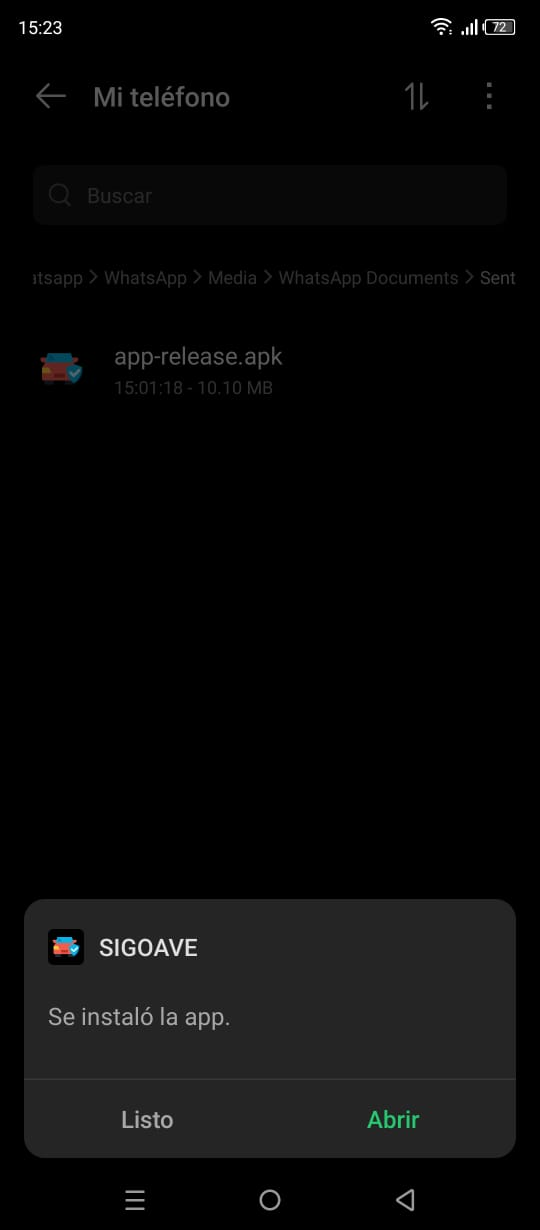
\includegraphics[width = 0.45\linewidth, height = 8.5cm]{14.jpeg}
		\caption{Instalación completa de la APP.}
	\end{figure}\\
	Dependiendo la configuración del usuario en el dispositivo, puede aparecer un mensaje emergente de control de seguridad. Ver Figura 15. En esta alerta se puede escoger cualquier opción como respuesta, pero se aconseja escoger la opción ``No Enviar'' para evitar que la Google Play detecte la APP como una posible amenaza.
	\begin{figure}[!h]
		\centering
		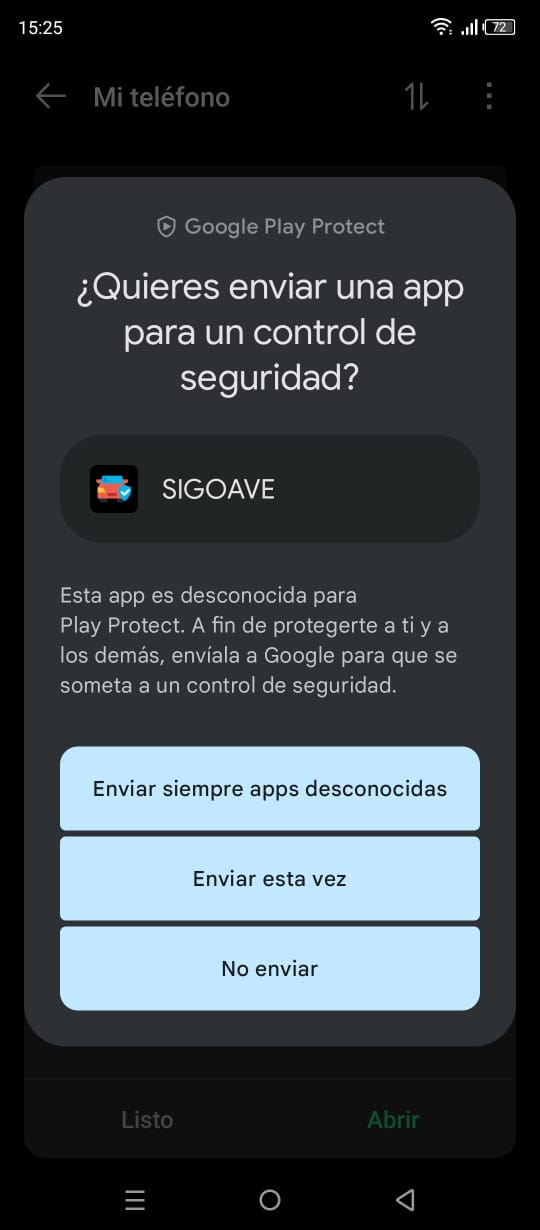
\includegraphics[width = 0.45\linewidth, height = 7.6cm]{15.jpeg}
		\caption{Control de seguridad Play Store Protect.}
	\end{figure}\\
	Finalmente, se puede apreciar la APP instalada en el dispositivo. Ver Figura 16.
	\begin{figure}[!h]
		\centering
		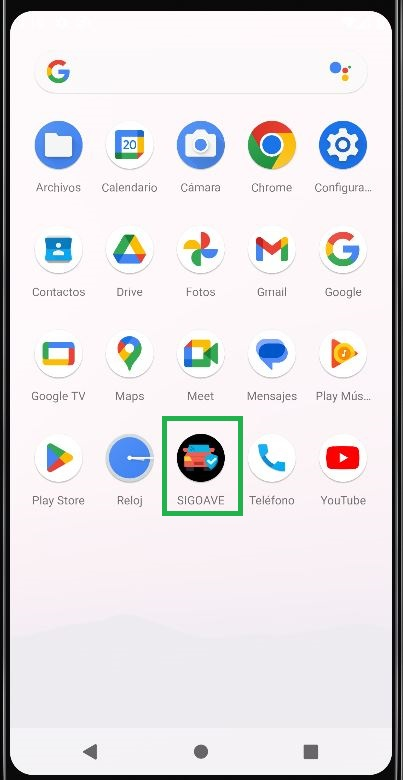
\includegraphics[width = 0.45\linewidth, height = 7.6cm]{16.jpg}
		\caption{APP instalada.}
	\end{figure}
	
	\section{Uso de la APP}
	El primer paso es iniciar la APP presionando sobre el icono de la misma, tras esto se abrirá la pantalla principal de la aplicación como se muestra en la Figura 17.
	\begin{figure}[!h]
		\centering
		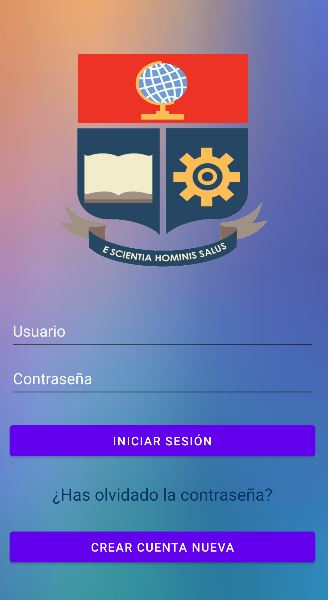
\includegraphics[width = 0.45\linewidth, height = 9cm]{17.jpg}
		\caption{Pantalla principal de la APP.}
	\end{figure}\\
	En esta pantalla tenemos tres opciones:
	\begin{itemize}
		\item Iniciar Sesión: permite ingresar a la APP como tal y hacer uso de todas sus funciones. Se necesita tener un usuario y una contraseña.
		\item Recuperar Contraseña: si el usuario ha olvidado sus credenciales (Contraseña) puede usar esta opción para restablecer una nueva contraseña.
		\item Crear Cuenta Nueva: permite a nuevos usuarios registrarse en la APP. 
	\end{itemize}

	\subsection{Crear Cuenta Nueva}
	Al presionar sobre el botón ``Crear Cuenta Nueva'' la aplicación redirigirá al usuario a una nueva interfaz como se muestra en la Figura 18.\\\\
	En esta interfaz se puede encontrar varios campos:
	\begin{itemize}
		\item Campos de Ingreso de Datos: representado por 4 campos. ``Correo Electrónico'', ``Nombre de Usuario'', ``Contraseña'' y ``Confirmar Contraseña''. Estos son los campos que el usuario debe llenar correctamente para crear una nueva cuenta.
		\item Limpiar: permite limpiar completamente los ``Campos de Ingreso de Datos'' l mismo tiempo.
		\item Cancelar: permite volver a la pantalla principal de la aplicación.
		\item Botón $\leftarrow$: permite volver a la pantalla principal de la aplicación. 
		\item Guardar: ingresado los ``Campos de Ingreso de Datos'' correctamente, crea un nuevo usuario de la aplicación.
	\end{itemize}
	\begin{figure}[!h]
		\centering
		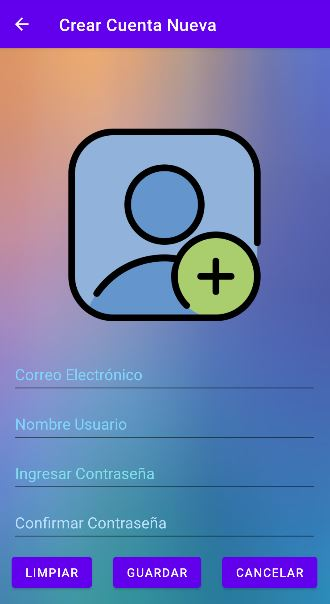
\includegraphics[width = 0.45\linewidth, height = 9cm]{18.jpg}
		\caption{Interfaz creación nuevo usuario.}
	\end{figure}
	En los campos que debe llenar el usuario se encuentra los campos:
	\begin{itemize}
		\item Correo Electrónico: debe ingresar un correo electrónico, valido y en formato adecuado (Ej: ejemplo@epn.edu.ec). A correo electrónico ingresado, posteriormente, se enviara un código de confirmación durante el registro del usuario.
		\item Nombre Usuario: en este campo se ingresara un nombre, fácil de recordar, con el cual el usuario posteriormente hará inicio de sesión. El nombre de usuario no debe tener espacios en blanco o caracteres especiales. Ver Figura 19.
		\item Ingresar Contraseña: la única condición de este parámetro es su longitud. La longitud mínima de la contraseña no puede ser menor a 8 caracteres. Ver Figura 19.
		\item Confirmar Contraseña: la única condición de este parámetro es su longitud y debe ser igual al campo ``Ingresar Contraseña''. La longitud mínima de la contraseña no puede ser menor a 8 caracteres. Ver Figura 19.
	\end{itemize}
	\begin{figure}[!ht]
		\centering
		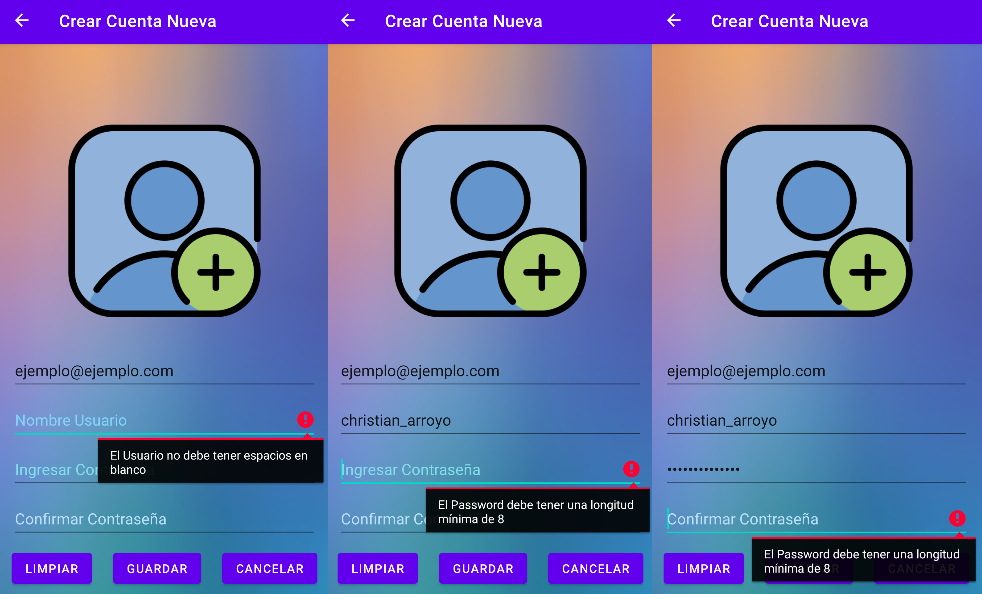
\includegraphics[width = 1\linewidth, height = 8.8cm]{19.png}
		\caption{Condiciones de los campos a llenar.}
	\end{figure}
	Si uno o varios de los parámetros esta erróneos se pueden presentar varias alertas como se muestra en la Figura 20.
	\begin{figure}[!ht]
		\centering
		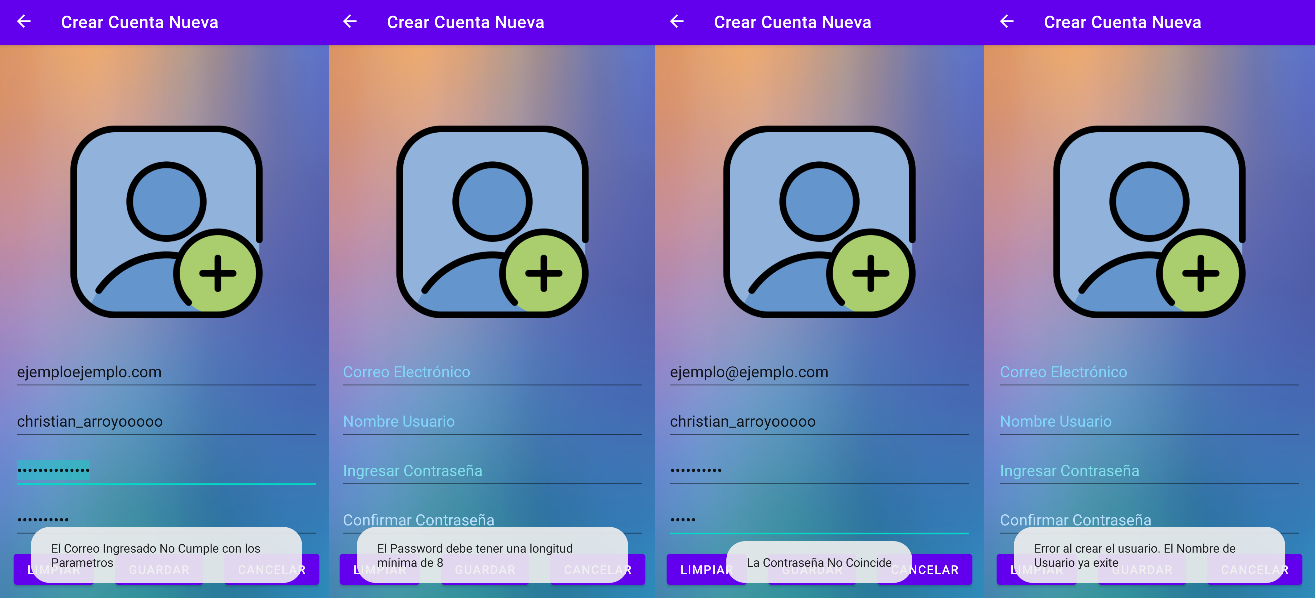
\includegraphics[width = 1\linewidth, height = 8.9cm]{20.png}
		\caption{Errores al crear u nuevo usuario.}
	\end{figure}\\
	Finalmente, tras llenar todos los campos de forma correcta y presionar el botón de ``Guardar'' la aplicación nos informara que se envió un código de confirmación al correo ingresado y redirigirá al usuario a una nueva interfaz. Ver Figura 21.
	\begin{figure}[!ht]
		\centering
		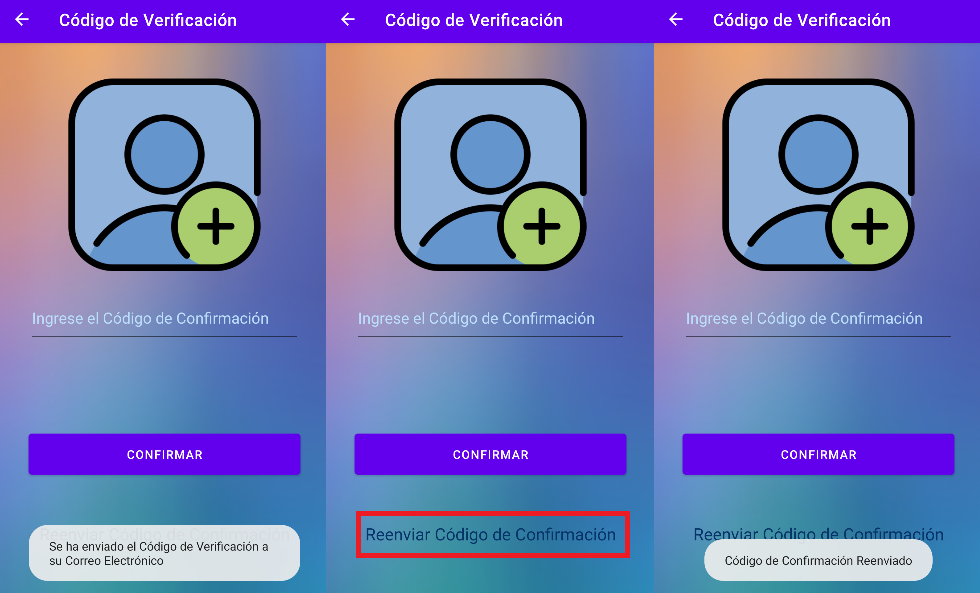
\includegraphics[width = 1\linewidth, height = 8.9cm]{21.png}
		\caption{Interfaz de Código de verificación.}
	\end{figure}\\
	En esta nueva interfaz se puede encontrar tres campos:
	\begin{itemize}
		\item Campo de Código Confirmación: en este campo se debe ingresar el Código de Confirmación que se envió a l correo del usuario. Este código en de tipo numérico.
		\item Este elemento permite  verificar que el campo de código no se encuentre vació y a la vez permite verificar que el código ingresado sea correcto.
		\item Reenviar Código: permite al usuario solicitar que se reenvié el código de confirmación si este no ha llegado al correo o si este código ha caducado. Recordar que el código de verificación tiene una duración de 5 minutos. Ver Figura 21, imagen central.
	\end{itemize}
	Si en usuario no ingresa el código de confirmación o si el código ingresado es incorrecto, recibirá unas alertas desde la APP informando de estas condiciones al usuario. Ver Figura 22.\\\\
	Al ingresar el código de confirmación y este ser verificado en el sistema se creara el nuevo usuario en el sistema, la aplicación informara de esto al usuario y finalmente, redirigirá al usuario a la interfaz principal. En la interfaz principal el usuario podrá iniciar sesión con las credenciales creadas anteriormente. Ver Figura 23.
	\begin{figure}[!ht]
		\centering
		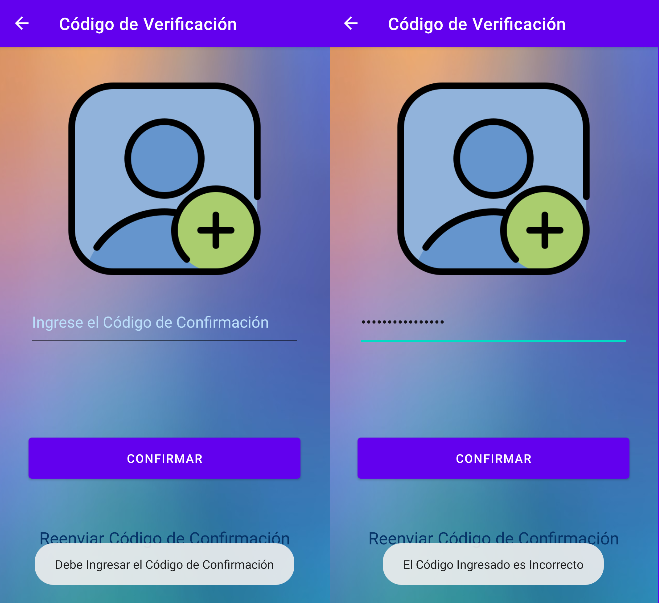
\includegraphics[width = .75\linewidth, height = 9cm]{22.png}
		\caption{Campo vació y código erróneo.}
	\end{figure}
	\begin{figure}[!ht]
		\centering
		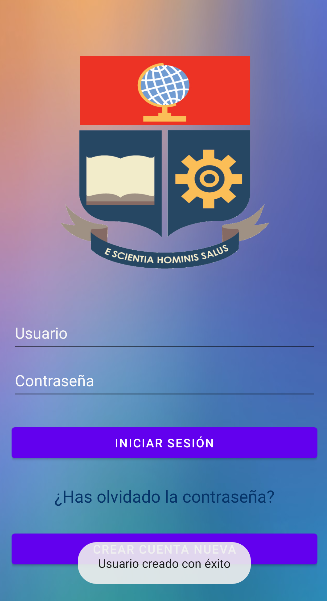
\includegraphics[width = .4\linewidth, height = 9cm]{23.png}
		\caption{Campo vació y código erróneo.}
	\end{figure}
		
	\subsection{Restablecer Contraseña}
	En la interfaz principal, ver Figura 17, se encuentra la opción de restablecer la contraseña de usuario. Al presionar en esta opción en la interfaz principal, la aplicación redirigirá al usuario a una nueva interfaz como se puede ver en la Figura 24.
	\begin{figure}[!ht]
		\centering
		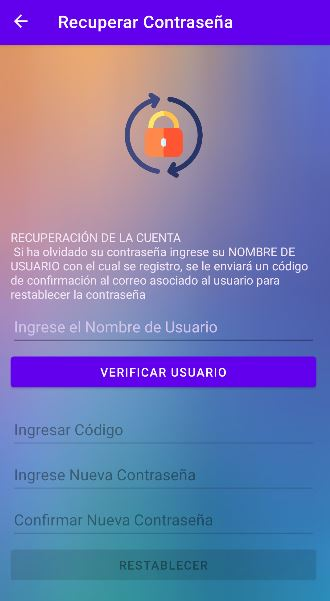
\includegraphics[width = .4\linewidth, height = 9cm]{24.jpg}
		\caption{Interfaz recuperación contraseña.}
	\end{figure}\\
	Para recuperar o cambiar la contraseña, el usuario debe ingresar su nombre de usuario y presionar el botón ``Verificar Usuario'', esto permitirá al sistema verificar la existencia del usuario.\\\\
	Si el usuario no existe se enviara un presentara una alerta como se ve en la Figura 25, caso contrario el sistema enviara un código de confirmación al correo asociado al nombre de usuario como se ve en la Figura 26.\\\\
	Recordar que se debe ingresar todos los campos de forma correcta. Si el usuario no ingresa de forma incorrecta los campos no se podrá restablecer la contraseña, como se ve en la Figura 27.Adicionalmente, recordar que la longitud de la contraseña no debe ser menor a 8 caracteres.\\\\
	Tras ingresar los datos solicitados de forma correcta y su comprobación en el sistema del código de confirmación, se restablecer la contraseña del usuario.\\\\
	La aplicación redirigirá al usuario a la interfaz principal para que pueda iniciar sesión con la nueva contraseña.
	\begin{figure}[!ht]
		\centering
		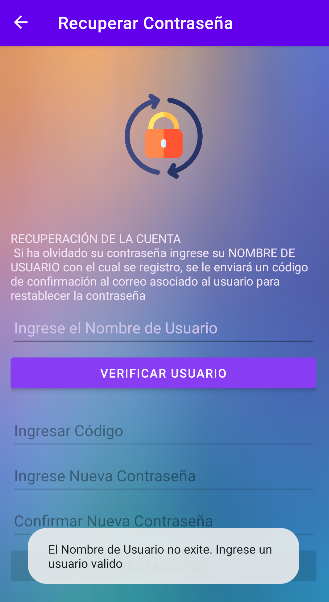
\includegraphics[width = .4\linewidth, height = 9cm]{25.png}
		\caption{Usuario ingresado erróneo.}
	\end{figure}
	\begin{figure}[!ht]
		\centering
		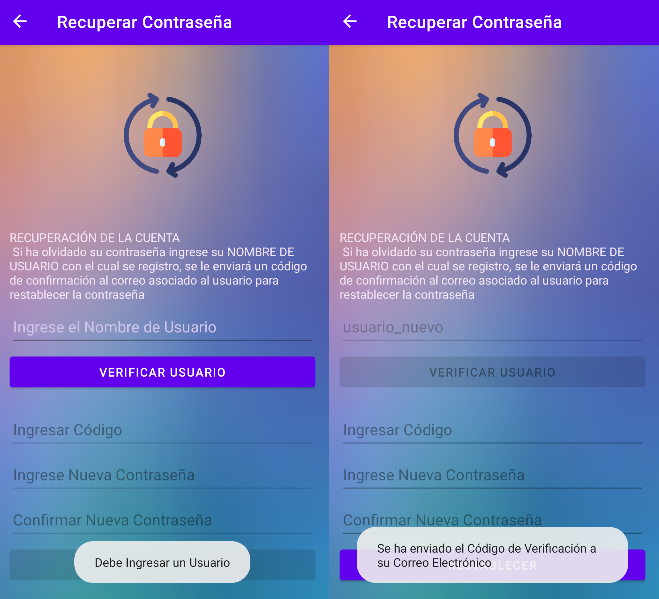
\includegraphics[width = .75\linewidth, height = 9cm]{26.png}
		\caption{Campo vació y usuario ingresado correcto.}
	\end{figure}
	\begin{figure}[!ht]
		\centering
		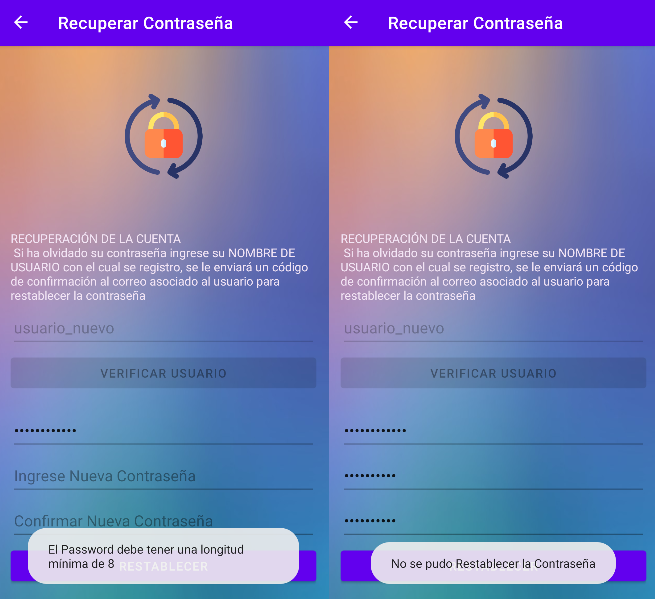
\includegraphics[width = .75\linewidth, height = 9cm]{27.png}
		\caption{Información incorrecta.}
	\end{figure}
	\begin{figure}[!ht]
		\centering
		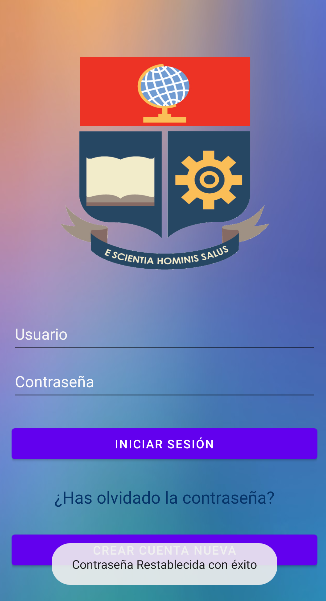
\includegraphics[width = .4\linewidth, height = 9cm]{28.png}
		\caption{Contraseña Restablecida.}
	\end{figure}
	
	\subsection{Iniciar Sesión}
	En la interfaz principal, el usuario deberá ingresar sus credenciales en los campos ``Usuario'' y ``Contraseña'' y luego presionar el botón ``Iniciar Sesión''. Si los campos están vacíos o incorrectos se mostrara un mensaje al usuario como se ve en la Figura 29. En la Figura 30 se muestra el inicio de sesión exitoso.
	\begin{figure}[!ht]
		\centering
		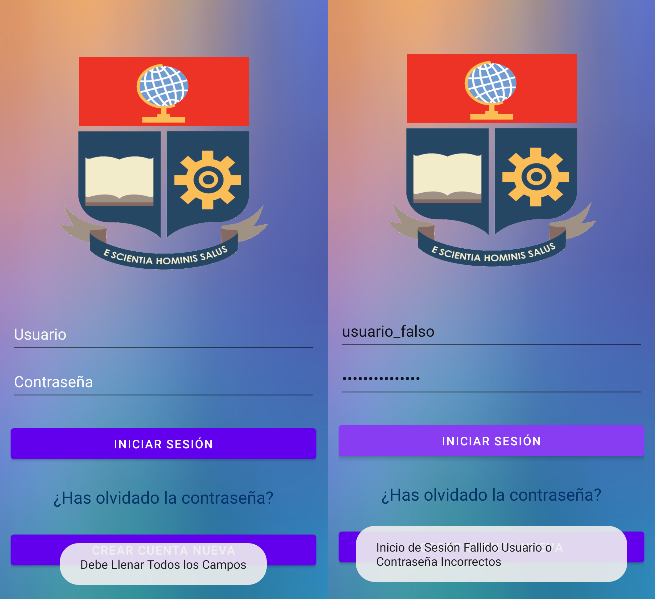
\includegraphics[width = .75\linewidth, height = 7.9cm]{29.png}
		\caption{Campos vacíos o credenciales incorrectas.}
	\end{figure}
	\begin{figure}[!ht]
		\centering
		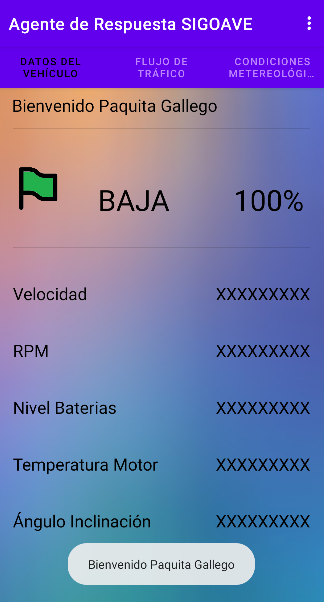
\includegraphics[width = .4\linewidth, height = 7.9cm]{30.png}
		\caption{Inicio de sesión correcto.}
	\end{figure}
	
	\subsection{Usando la Aplicación}
	Iniciada la sesión se mostrara una interfaz compuesta por varias partes, ver Figura 31, que se detallan a continuación:
	\begin{itemize}
		\item Cabecera: Muestra el nombre de la APP como ``Agente de Respuesta SIGOAVE''.
		\item Información principal del vehículo, dividido en tres secciones:
		\begin{itemize}
			\item Datos del vehículo: se presenta información como: velocidad, RPM, nivel de batería, temperatura del motor y ángulo de inclinación.
			\item Flujo de Trafico: se presenta información como: ubicación, velocidad promedio, número de vehículos, ocupación promedio, dirección del flujo.
			\item Condiciones meteorológicas: se presenta información como: lugar, temperatura precipitación, humedad y velocidad del viento.
		\end{itemize}
		\item Nombre de usuario: presentado como ``Bienvenido'' $+$ ``Nombre$\_$Usuario''.
		\item Bandera de alerta: puede presentar cuatro niveles de alerta: verde, amarilla, naranja y rojo.
		\item Frase de alerta: puede presentar cuatro niveles de alerta: baja, media, alta y muy alta.
		\item Porcentaje de alerta: dependerá del nivel de alerta, varia entre 0 y 100 por ciento.
		\item Botón de mapas: redirigirá al usuario a la función de mapas.
		\item Botón de usuario: redirigirá al usuario a las configuraciones del usuario.
		\item Botón de comentarios: redirigirá al usuario al la función de correo que permite la comunicación entre el usuario y los desarrolladores de la APP.
	\end{itemize}
	Esta interfaz tiene comunicación con el vehículo, desde el vehículo se extrae la información que se presenta en la interfaz de usuario, esta información a la vez es enviada al agente de respuesta que esta anidado en AWS para su análisis. Una vez analizada la información esta es devuelta al dispositivo del usuario donde se presentaran las alertas según su nivel.\\\\
	Las alerta pueden ser de 4 niveles, empezando desde la más baja:
	\begin{itemize}
		\item Alerta Verde: alerta baja, niveles normales, no representa riesgo. Ver Figura 32.
		\item Alerta Amarilla: alerta media, niveles un poco altos, no representa riesgo pero se debe estar alerta. Ver Figura 32.
		\item Alerta Naranja: alerta alta, niveles altos, representa riesgo de accidente. Ver Figura 32.
		\item Alerta Roja: alerta muy alta, niveles muy altos, enorme riesgo de accidente. Ver Figura 32.
	\end{itemize}
	Las alertas son visuales y sonoras. Estas alertas tienen un temporizador de 5 segundos, después de lo cual las misma se descartan automáticamente.
	\begin{figure}[!ht]
		\centering
		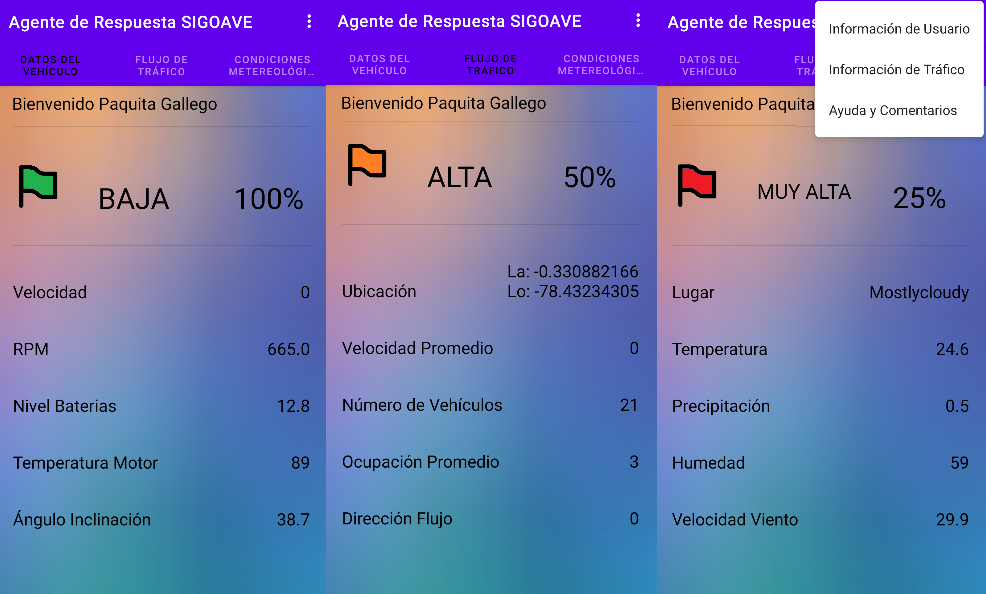
\includegraphics[width = 1\linewidth, height = 9cm]{31.png}
		\caption{Partes de la interfaz de la APP.}
	\end{figure}
	\begin{figure}[!ht]
		\centering
		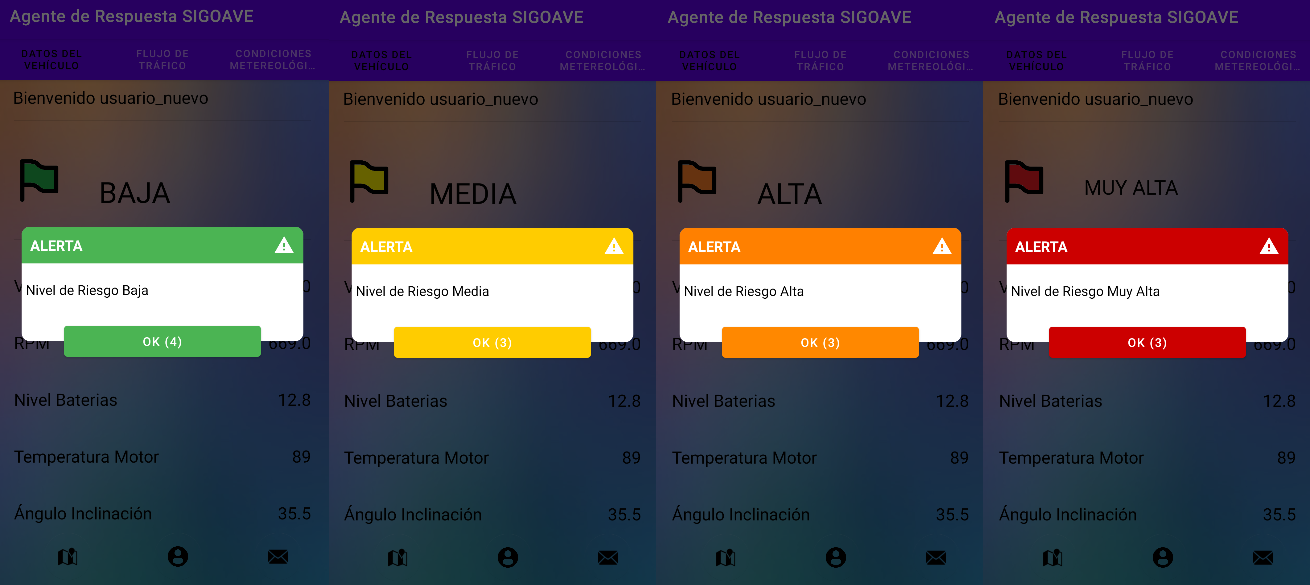
\includegraphics[width = 1\linewidth, height = 9cm]{32.png}
		\caption{Niveles de Alerta.}
	\end{figure}
	
	\subsection{Mapas}
	Al presionar el botón de mapas la aplicación enviara al usuario a la interfaz de mapas, en esta interfaz el usuario podrá ver su ubicación actual en un mapa y a su vez podrá ver información del trafico cercano a su ubicación. Antes de usar la sección de mapas el usuario debe proporcionar los permisos necesarios, como se ve en la Figura 33. En la misma interfaz se puede alternar entre dos formas de vista: modo satélite y modo capas. Como se ve en la Figura 34.
	\begin{figure}[!ht]
		\centering
		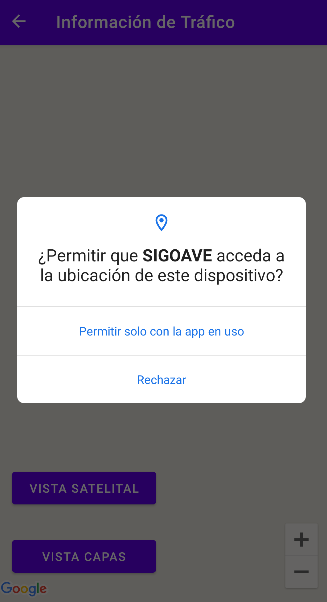
\includegraphics[width = 0.4\linewidth, height = 7.5cm]{33.png}
		\caption{Permisos de Aplicación.}
	\end{figure}
	\begin{figure}[!ht]
		\centering
		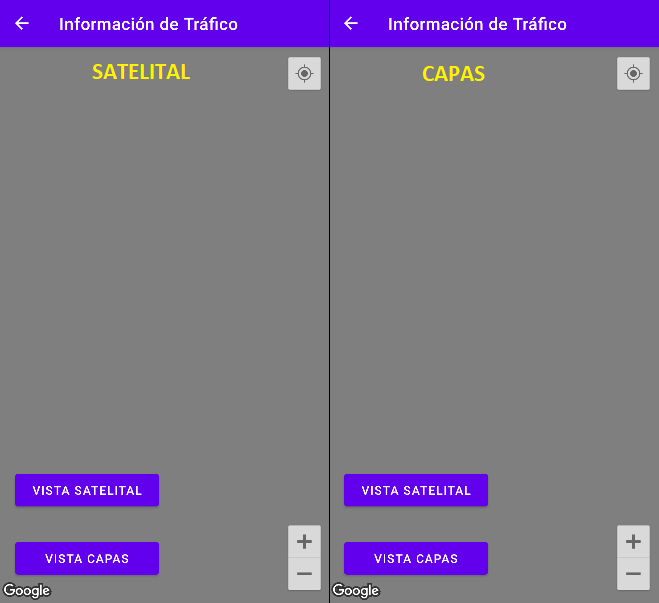
\includegraphics[width = 0.6\linewidth, height = 7.5cm]{34.png}
		\caption{Vista de Mapas.}
	\end{figure}
	
	\subsection{Comentarios}
	Interfaz que permite la comunicación entre el usuario de la APP y los desarrolladores de la APP. Ver Figura 35. En este apartado el usuario podrá ingresar un titulo y un comentario, después de lo cual deberá presionar el botón ``Enviar Comentario'', lo cual enviara al usuario a una nueva pantalla donde podrá escoger el servidor de correo deseado con el cual enviar un correo. Ver Figura 36.
	\begin{figure}[!ht]
		\centering
		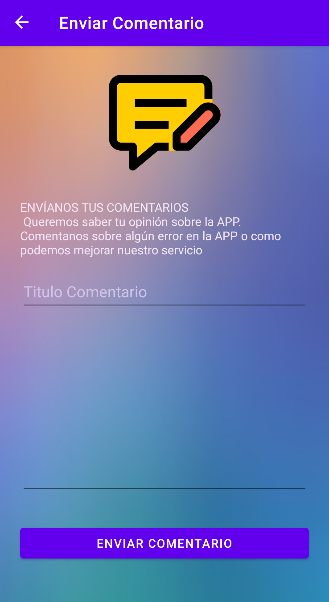
\includegraphics[width = 0.4\linewidth, height = 7.5cm]{35.png}
		\caption{Sección Comentarios.}
	\end{figure}
	\begin{figure}[!ht]
		\centering
		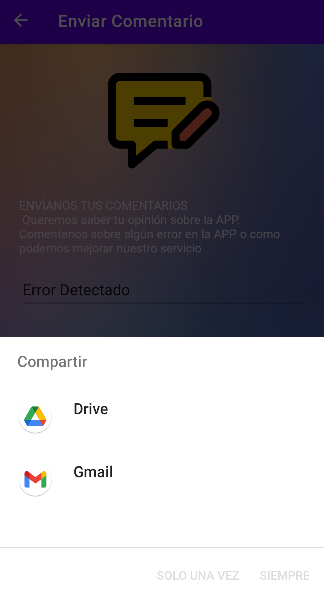
\includegraphics[width = 0.4\linewidth, height = 7.5cm]{36.png}
		\caption{Elección de Correo.}
	\end{figure}
	
	\subsection{Configuración de Usuario}
	En esta sección se presenta el perfil del usuario. Se muestra información pertinente al usuario de la aplicación. En este apartado el usuario podrá modificar o eliminar parámetros de la cuenta. Ver Figura 37 y 38.
	\begin{figure}[!ht]
		\centering
		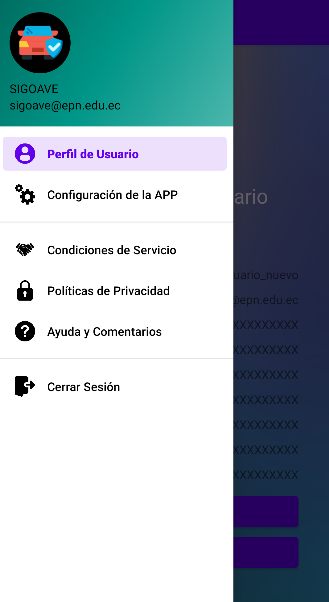
\includegraphics[width = 0.4\linewidth, height = 8.1cm]{37.png}
		\caption{Perfil de usuario.}
	\end{figure}
	\begin{figure}[!ht]
		\centering
		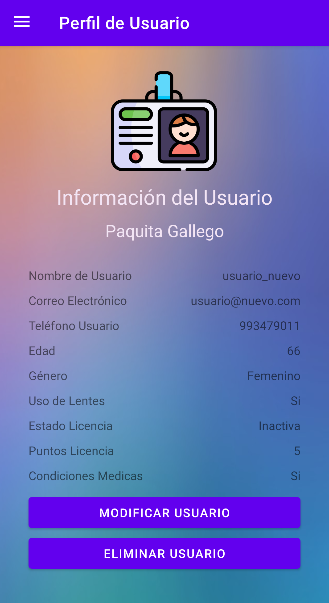
\includegraphics[width = 0.4\linewidth, height = 8.1cm]{38.png}
		\caption{Parámetros de la cuenta.}
	\end{figure}\\
	\subsubsection{Modificar Usuario}
	Dentro de este apartado se puede modificar o agregar información del usuario a la base de datos. En la Figura 39, se muestra un usuario sin datos agregados en la base de datos, solo se muestra información básica que se agrego al momento de crear el usuario.
	\begin{figure}[!ht]
		\centering
		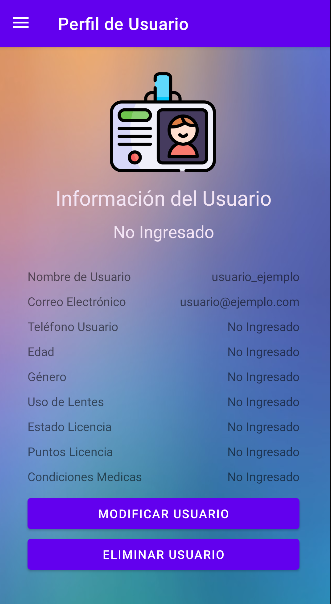
\includegraphics[width = 0.4\linewidth, height = 8.1cm]{39.png}
		\caption{Usuario sin agregar información.}
	\end{figure}\\
	Para modificar o agregar datos al usuario se debe presionar en el botón ``Modificar Usuario'', después de lo cual se presentara una nueva pantalla donde se mostrara la información que se puede agregar. En la Figura 40 se muestra la interfaz cuando ya se encuentra agregada la información y en la Figura 41 se muestra la interfaz cuando aún no se encuentra agregada la información del usuario.\\\\
	En esta interfaz el usuario puede escoger entre una serie de opciones para agregar o modificar sus datos, estas opciones son:
	\begin{itemize}
		\item Nombre del Cliente: de tipo texto, no se aceptan números o espacios.
		\item Apellido del Cliente: de tipo texto, no se aceptan números o espacios.
		\item Nombre de usuario: de tipo texto, no se puede modificar, ingresado al momento de crear el usuario.
		\item Correo Electrónico: de tipo alfanumérico, no se puede modificar directamente, ingresado al momento de crear el usuario. Si se desea modificar se debe contactar con el administrador de la APP.
		\item Teléfono Usuario: de tipo numérico, no se acepta letra o espacios.
		\item Edad: de tipo numérico, se puede escoger entre un rango de 00 a 100.
		\item Género: de tipo texto, se puede escoger entre dos opciones: ``Masculino'' y ``Femenino''.
		\item Uso Lentes: de tipo texto, se puede escoger entre dos opciones: ``Si'' y ``No''.
		\item Estado Licencia: de tipo texto, se puede escoger entre dos opciones: ``Activa'' e ``Inactiva''.
		\item Puntos Licencia: de tipo numérico, se puede escoger entre un rango de 00 a 30.
		\item Condiciones Medicas: de tipo texto, se puede escoger entre dos opciones: ``Si'' y ``No''.
	\end{itemize}
	\begin{figure}[!ht]
		\centering
		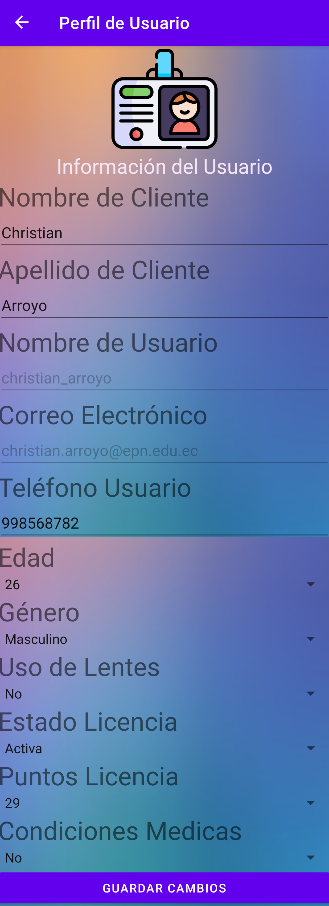
\includegraphics[width = 0.4\linewidth, height = 13.2cm]{40.png}
		\caption{Usuario con datos agregados.}
	\end{figure}
	\begin{figure}[!ht]
		\centering
		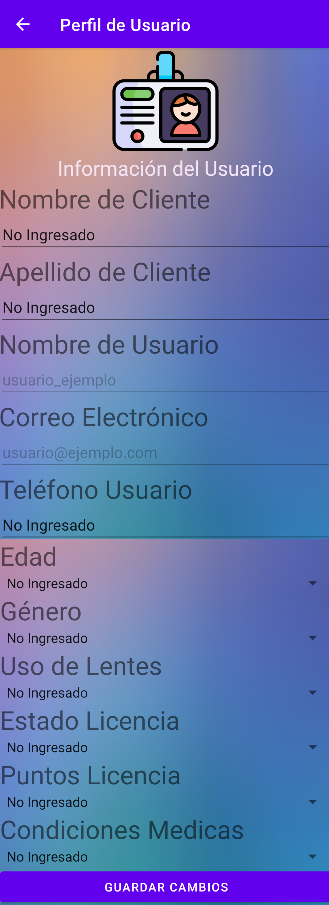
\includegraphics[width = 0.4\linewidth, height = 8.1cm]{41.png}
		\caption{Usuario sin datos agregados.}
	\end{figure}
	Se debe cerciorar que se ingresaron todos los datos, caso  contrario se presentara un mensaje de alerta al momento de tratar de ingresar los datos como se muestra en la Figura 42. Si el usuario ingreso los datos correctamente y al presionar el botón ``Guardar Cambios'' se retornara a la interfaz principal y se mostrara un mensaje de información como muestra la Figura 43.
	\begin{figure}[!ht]
		\centering
		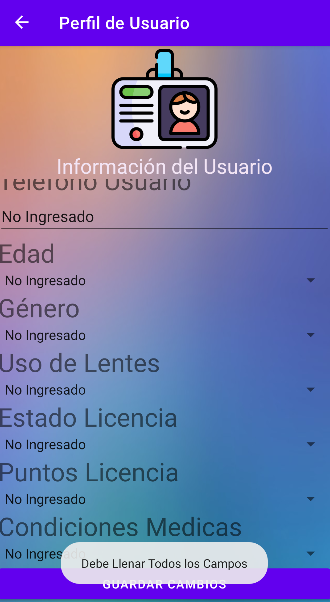
\includegraphics[width = 0.4\linewidth, height = 8.1cm]{42.png}
		\caption{Error al no ingresar todos los datos.}
	\end{figure}
	\begin{figure}[!ht]
		\centering
		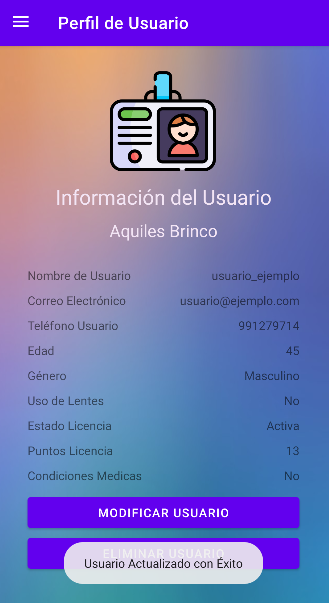
\includegraphics[width = 0.4\linewidth, height = 8.3cm]{43.png}
		\caption{Usuario Actualizado.}
	\end{figure}

	\subsubsection{Eliminar Usuario}
	En la interfaz principal se encuentra la opción de ``Eliminar Usuario'', ver Figura 44. 
	\begin{figure}[!ht]
		\centering
		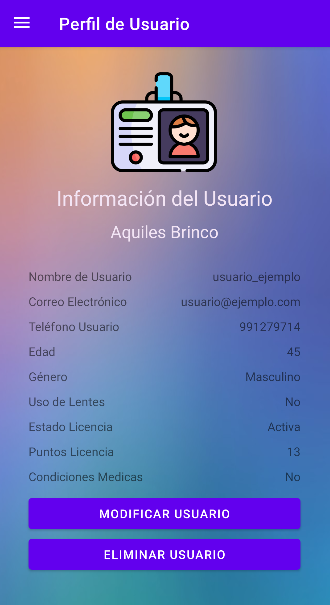
\includegraphics[width = 0.4\linewidth, height = 8.3cm]{44.png}
		\caption{Eliminar Usuario.}
	\end{figure}\\
	Al presionar el botón ``Eliminar Usuario'' se presentara un mensaje de alerta en el cual se pedirá confirmar la eliminación del usuario como se muestra en la Figura 45. Este mensaje tendrá una duración de 5 segundos, tiempo durante el cual el usuario debe presionar el botón ``Ok'' para eliminar el usuario. Si el usuario no desea eliminar debe dejar pasar los 5 segundos para que el mensaje se descarte automáticamente o presionar en cualquier parte de la pantalla fuera del cuadro del mensaje de alerta.
	\begin{figure}[!ht]
		\centering
		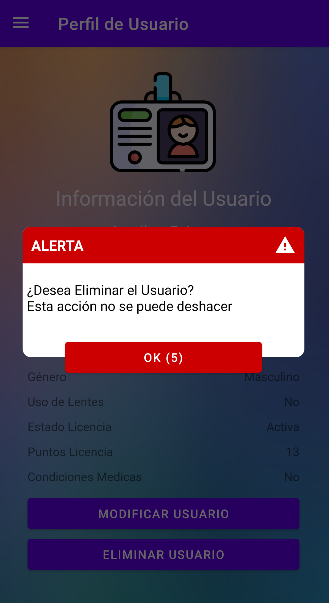
\includegraphics[width = 0.4\linewidth, height = 7cm]{45.png}
		\caption{Mensaje de Advertencia.}
	\end{figure}\\
	Si el usuario presiona ``Ok'' en el mensaje de alerta, se procederá a eliminar la cuenta y se redirigirá al usuario a la interfaz de inicio de sesión, ver Figura 46. Recordar que esto es irreversible.
	\begin{figure}[!ht]
		\centering
		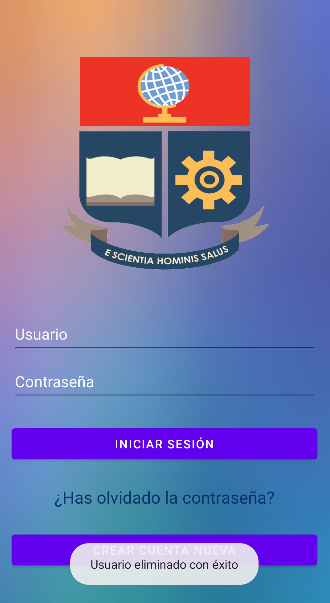
\includegraphics[width = 0.4\linewidth, height = 6.9cm]{46.png}
		\caption{Usuario Eliminado.}
	\end{figure}
	
	\subsubsection{Parámetros Cuenta de Usuario}
	Dentro de los parámetros de la cuenta de usuario se encuentran (ver Figura 47):
	\begin{itemize}
		\item Perfil de Usuario: muestra información básica del usuario como: nombre, correo, teléfono, edad, etc.
		\item Configuración de la APP: permite configurar las alerta a presentar de la APP.
		\item Condiciones de servicios: información sobre el uso de la APP.
		\item Políticas de Privacidad: información sobre el uso de la APP.
		\item Ayuda y Comentarios: permite la comunicación con los desarrolladores, ver sección comentarios.
		\item Cerrar Sesión: permite cerrar la sesión actual del usuario, después de lo cual deberá volver a iniciar sesión.
	\end{itemize}
	\begin{figure}[!ht]
		\centering
		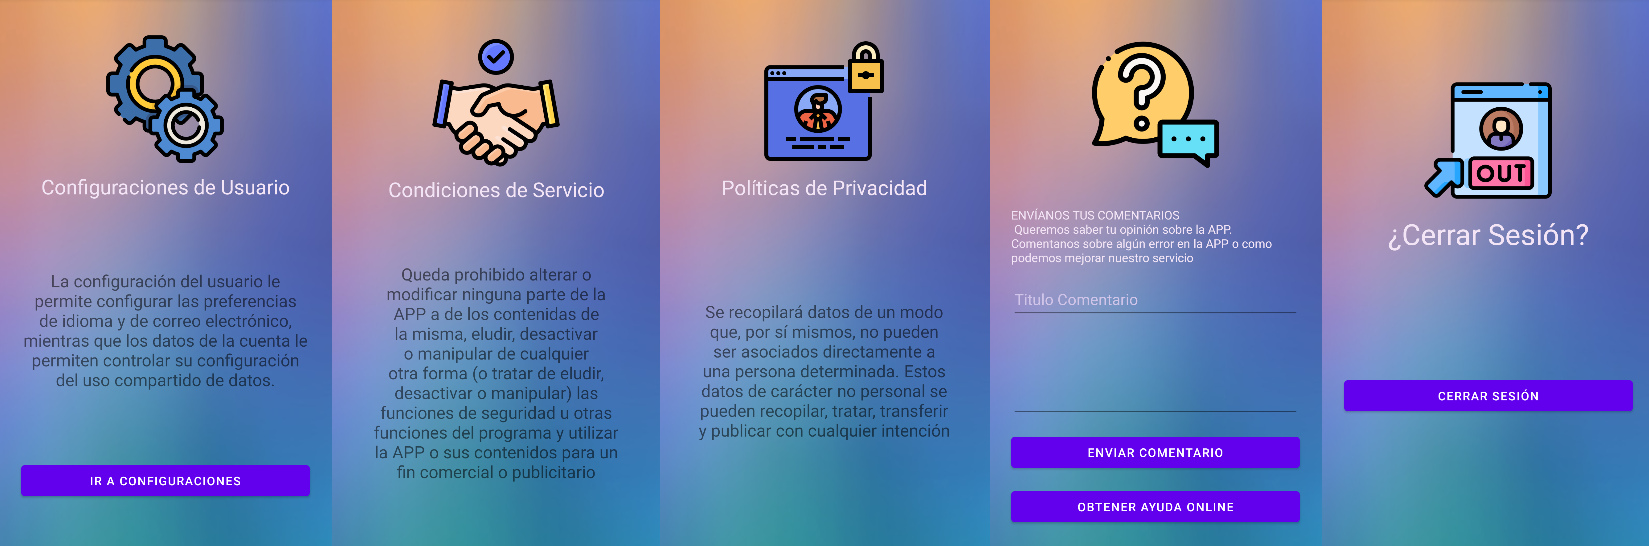
\includegraphics[width = 1\linewidth, height = 9.8cm]{47.png}
		\caption{Parámetros de la cuenta.}
	\end{figure}
	La sección de ``Configuración de Usuario'' permite configurar las alertas que se desea mostrar al usuario, es decir, permite configurar si se desea mostrar solo alertas bajas, medias, altas, muy altas o un combinación de estas como se muestra en la Figura 48. Una vez escogida las alertas que se desea mostrar se presiona en ``Guardar Configuración'' lo cual redirigirá al perfil de usuario.
	\begin{figure}[!ht]
		\centering
		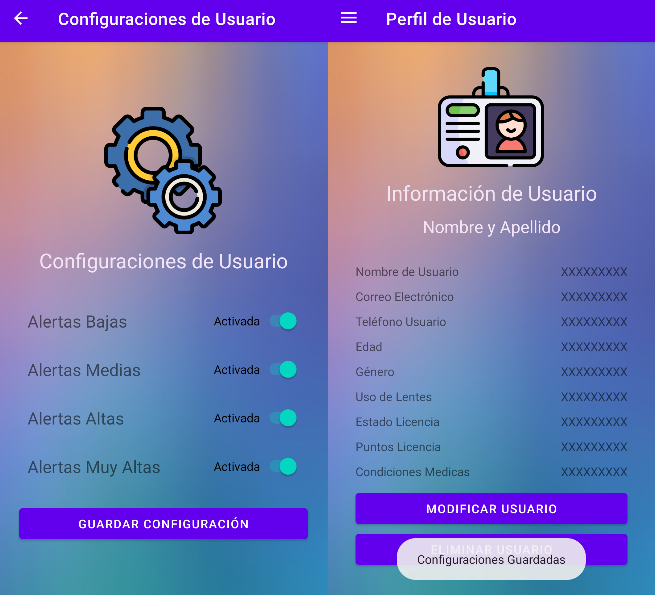
\includegraphics[width = 0.60\linewidth, height = 8.5cm]{48.png}
		\caption{Configuración de alertas.}
	\end{figure}
	La sección cerrar cuenta, permite cerrar la sección actual. En este apartado se presentara un mensaje de alerta al usuario que informara que esta apunto de cerrar sesión, como se ve en la Figura 49.
	\begin{figure}[!ht]
		\centering
		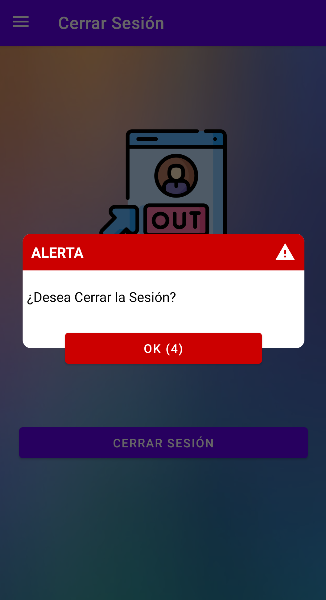
\includegraphics[width = 0.4\linewidth, height = 8.5cm]{49.png}
		\caption{Cerrando sesión de usuario.}
	\end{figure}\\
	Este mensaje tiene una duración de 5 segundos después de lo cual se descarta automáticamente si el usuario no realiza ninguna acción. Si el usuario presiona en el botón ``OK'' antes de que el tiempo se acabe se cerrar la sesión actual del usuario. Se informara al usuario del cierre de sesión y se redirigirá al usuario a la interfaz principal de la APP. Ver Figura 50.
	\begin{figure}[!ht]
		\centering
		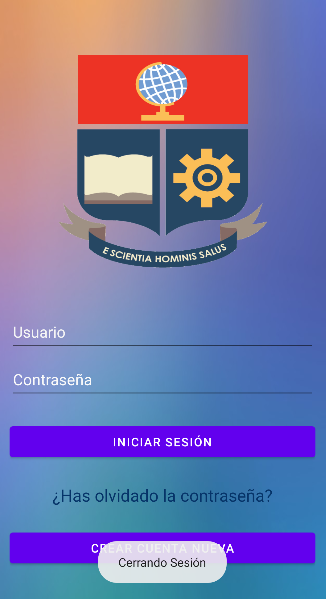
\includegraphics[width = 0.4\linewidth, height = 8.1cm]{50.png}
		\caption{Cierre de sesión exitoso.}
	\end{figure}
	
	\section{Conclusiones}
	\begin{itemize}
		\item Se mostró la interfaz gráfica de usuario de la aplicación móvil del agente de respuesta.
		\item Se establecieron mejoras a funcionalidades existentes y funcionalidades nuevas para la aplicación.
		\item Se consideraron en la fase de desarrollo e implementación, los riesgos de seguridad definidos en la fase de diseño.
	\end{itemize}	
\end{document}